\subsection{MIT-Access Card}

MIT card inculde both a magnetic strip and an RFID tag (125 kHz).
An analysis showed that eavesdropping twice the communication 
reveals the same broadcast.
\begin{itemize}
	\item Broadcast contains 224bits 
	\item with only 32 bits variying form card
	to card
\end{itemize}
An attack can be done by replaying a recording of a previously broadcasted value.

\subsection{EMV-CAP}

Used by bank to authenticate customers online 
\begin{itemize}
	\item Mode 1 : Authentication to get access to an e-banking account 
	\begin{center}
		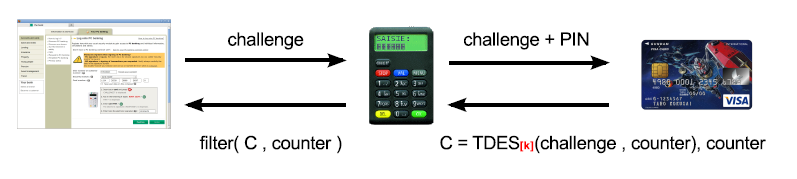
\includegraphics[scale=0.6]{img/mode1-ebanking}
	\end{center}
	
	\item Mode 2 : Signature of a financial transaction
	\begin{center}
		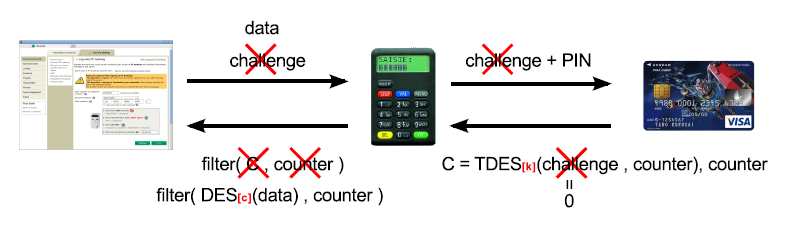
\includegraphics[scale=0.6]{img/mode2-ebanking}
	\end{center}
\end{itemize}
The first mode is secure but with the second replay attack is possible. %preplay too?

\subsection{Digital Signature Transponder}

Texas Instruments Digital Signature Transponder is a tag used to enable 
fuel-injection system of the vehicle.
\begin{itemize}
	\item It uses a Proprietary cipher that uses 40-bit keys
	\item DST responses to 8 queries per second.
\end{itemize}
Authentication:
\begin{tabular}{m{8cm}m{6cm}}
\begin{eqnarray*}
	Verifier \rightarrow Prover & r\\
	Verifier \leftarrow Prover & id,Trunc_{24}(E_k(r)),checksum \\
\end{eqnarray*}
&
\begin{itemize}
	\item |k| = |r| = |$E_k(r)$| = 40bits
	\item |identifier| = |$Truncate_{24}(E_k(r))$| = 24 bits
	\item |checksum| = 16 bits
\end{itemize}
\end{tabular}
An attack has been perfomed on this system which consist of:
\begin{enumerate}
	\item Reverse enginneering the cipher
	\item Eavesdropping some communications
	\item Recovering the key using a brute force attack
	\item Simulating the tag to ignit the targeted tag
\end{enumerate}
\paragraph{Security}
\begin{itemize}
	\item Because the tag respond to any challenge, it's possible to challenge it instead
	of eavesdropping it
	\item Since the tag response is truncated, using a brute force on one 
	challenge/response pair leads to several possible keys ( pigeonhole principle)
	\item Authors managed to recover a key with 16 FGPAs in parallel
\end{itemize}
